\documentclass[bachelor, och, labwork]{shiza}
% параметр - тип обучения - одно из значений:
%    spec     - специальность
%    bachelor - бакалавриат (по умолчанию)
%    master   - магистратура
% параметр - форма обучения - одно из значений:
%    och   - очное (по умолчанию)
%    zaoch - заочное
% параметр - тип работы - одно из значений:
%    referat    - реферат
%    coursework - курсовая работа (по умолчанию)
%    diploma    - дипломная работа
%    pract      - отчет по практике
% параметр - включение шрифта
%    times    - включение шрифта Times New Roman (если установлен)
%               по умолчанию выключен
\usepackage{subfigure}
\usepackage{tikz,pgfplots}
\pgfplotsset{compat=1.5}
\usepackage{float}

%\usepackage{titlesec}
\setcounter{secnumdepth}{4}
%\titleformat{\paragraph}
%{\normalfont\normalsize}{\theparagraph}{1em}{}
%\titlespacing*{\paragraph}
%{35.5pt}{3.25ex plus 1ex minus .2ex}{1.5ex plus .2ex}

\titleformat{\paragraph}[block]
{\hspace{1.25cm}\normalfont}
{\theparagraph}{1ex}{}
\titlespacing{\paragraph}
{0cm}{2ex plus 1ex minus .2ex}{.4ex plus.2ex}

% --------------------------------------------------------------------------%


\usepackage[T2A]{fontenc}
\usepackage[utf8]{inputenc}
\usepackage{graphicx}
\graphicspath{ {./images/} }
\usepackage{tempora}

\usepackage[sort,compress]{cite}
\usepackage{amsmath}
\usepackage{amssymb}
\usepackage{amsthm}
\usepackage{fancyvrb}
\usepackage{listings}
\usepackage{listingsutf8}
\usepackage{longtable}
\usepackage{array}
\usepackage[english,russian]{babel}

% \usepackage[colorlinks=true]{hyperref}
\usepackage{url}

\usepackage{underscore}
\usepackage{setspace}
\usepackage{indentfirst} 
\usepackage{mathtools}
\usepackage{amsfonts}
\usepackage{enumitem}
\usepackage{tikz}

\newcommand{\eqdef}{\stackrel {\rm def}{=}}
\newcommand{\specialcell}[2][c]{%
\begin{tabular}[#1]{@{}c@{}}#2\end{tabular}}

\renewcommand\theFancyVerbLine{\small\arabic{FancyVerbLine}}

\newtheorem{lem}{Лемма}

\begin{document}

% Кафедра (в родительном падеже)
\chair{}

% Тема работы
\title{ОCНОВЫ IP- АДРКСАЦИИ. ПОДСЕТИ СЕТЕЙ РАЗЛИЧНЫХ КЛАССОВ}

% Курс
\course{2}

% Группа
\group{231}

% Факультет (в родительном падеже) (по умолчанию "факультета КНиИТ")
\department{факультета КНиИТ}

% Специальность/направление код - наименование
%\napravlenie{09.03.04 "--- Программная инженерия}
%\napravlenie{010500 "--- Математическое обеспечение и администрирование информационных систем}
%\napravlenie{230100 "--- Информатика и вычислительная техника}
%\napravlenie{231000 "--- Программная инженерия}
\napravlenie{100501 "--- Компьютерная безопасность}

% Для студентки. Для работы студента следующая команда не нужна.
% \studenttitle{Студентки}

% Фамилия, имя, отчество в родительном падеже
\author{Окунькова Сергея Викторовича}

% Заведующий кафедрой
% \chtitle{} % степень, звание
% \chname{}

%Научный руководитель (для реферата преподаватель проверяющий работу)
\satitle{ассистент} %должность, степень, звание
\saname{А. А. Фомин}

% Руководитель практики от организации (только для практики,
% для остальных типов работ не используется)
% \patitle{к.ф.-м.н.}
% \paname{С.~В.~Миронов}

% Семестр (только для практики, для остальных
% типов работ не используется)
%\term{8}

% Наименование практики (только для практики, для остальных
% типов работ не используется)
%\practtype{преддипломная}

% Продолжительность практики (количество недель) (только для практики,
% для остальных типов работ не используется)
%\duration{4}

% Даты начала и окончания практики (только для практики, для остальных
% типов работ не используется)
%\practStart{30.04.2019}
%\practFinish{27.05.2019}

% Год выполнения отчета
\date{2021}

\maketitle

% Включение нумерации рисунков, формул и таблиц по разделам
% (по умолчанию - нумерация сквозная)
% (допускается оба вида нумерации)
% \secNumbering

%-------------------------------------------------------------------------------------------
\tableofcontents

\section{Задание 1}

\begin{enumerate}
    \item Вычислите адреса сетей хостов X и Z. 
    
    \begin{figure}[H]
        \centering      %размер рисунка       здесь находится название файла рисунка, без указания формата
        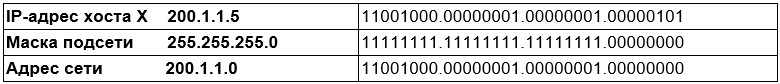
\includegraphics[width=1\textwidth]{1}
        \label{fig:image1}
    \end{figure}

    \begin{figure}[H]
        \centering      %размер рисунка       здесь находится название файла рисунка, без указания формата
        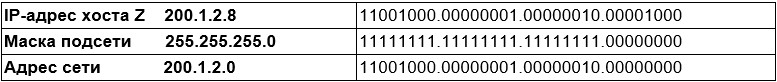
\includegraphics[width=1\textwidth]{2}
        \label{fig:image1}
    \end{figure}
    
    Ответ: Адресс сети хоста X = 200.1.1.0, адресс сети хоста Y = 200.1.2.0
    
    \item Находятся ли хосты X и Z в одной сети класса С? 
    
    Ответ: нет
\end{enumerate}

\section{Задание 2}

\begin{enumerate}
    
    \item Заполните таблицу для 4 подсетей сети класса С c маской 255.255.255.192
    
    \begin{figure}[H]
        \centering      %размер рисунка       здесь находится название файла рисунка, без указания формата
        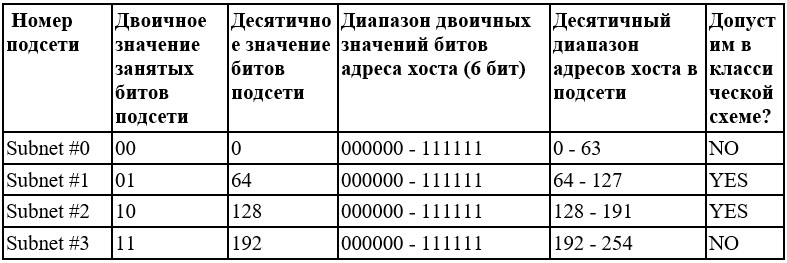
\includegraphics[width=1\textwidth]{3}
        \label{fig:image1}
    \end{figure}

\end{enumerate}

\section{Задание 3}

Вам выделена сеть класса B с адресом 150.193.0.0. Необходимо разбить ее не менее, чем на 50 подсетей. В каждой из подсетей должно быть не менее 750 адресов хостов.

\begin{enumerate}

    \item Запишите двоичный эквивалент адреса 150.193.0.0?
    
    Ответ: 10010110.11000001.00000000.00000000
    \item Какие октеты и сколько бит используется для адресации сети в этом адресе?
    
    Ответ: первые 2 октета, 16 бит
    \item Сколько хостов можно адресовать в сети класса В? 
    
    Ответ:65 534
    \item Сколько бит следует занять из части адреса, относящейся к хостам, для того, чтобы получить в сети класса В не меньше 50 подсетей, при чем в каждой не менее, 
    чем по 750 адресов хостов?

    Ответ: 6 бит
    \item Какую маску подсети в двоичном представлении вы используете при заданном разбиении?
    
    Ответ: 11111111.11111111.00000000.00000000
    \item Запишите десятичный эквивалент этой маски: 
    
    Ответ: 255.255.0.0
    \item Заполните таблицу  для первых семи из возможных подсетей сети класса B 150.193.0.0, полученных заимствованием 6 битов из третьего октета адреса.
    
    \begin{figure}[H]
        \centering      %размер рисунка       здесь находится название файла рисунка, без указания формата
        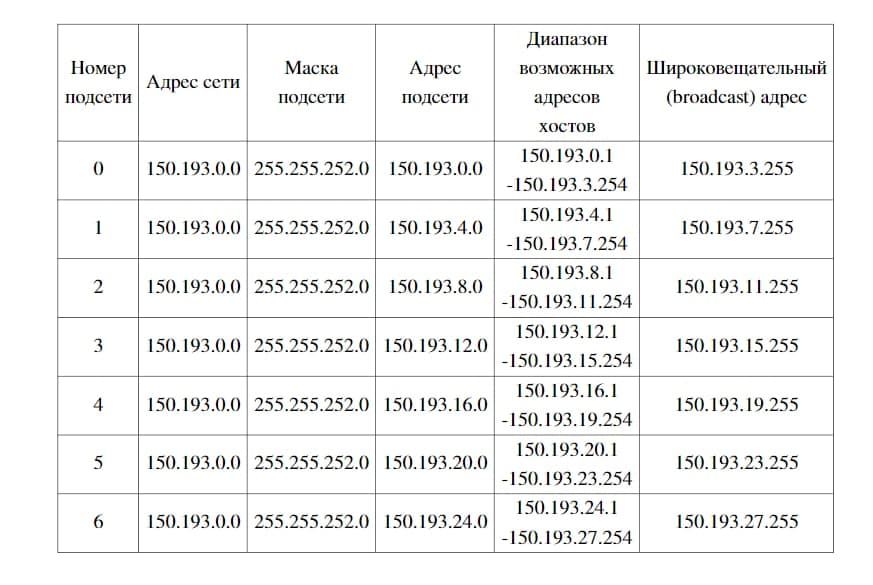
\includegraphics[width=1\textwidth]{4}
        \label{fig:image1}
    \end{figure}

    \item На рисунке приведена схема сети, состоящая из 3 сегментов. Используя построенный для сети 150.193.0.0 адресный план, заполните пропущенные значения адресов и масок.
    
    \begin{figure}[H]
        \centering      %размер рисунка       здесь находится название файла рисунка, без указания формата
        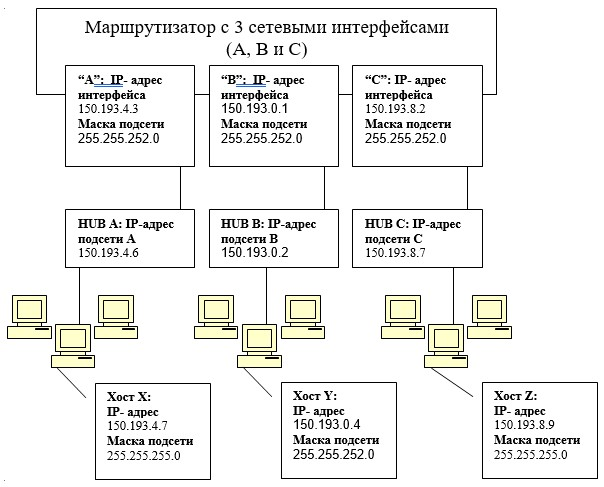
\includegraphics[width=1\textwidth]{5}
        \label{fig:image1}
    \end{figure}

    \item Опишите по шагам процесс передачи пакета от хоста X к хосту Z в сети на рисунке.
    
    Ответ: хост X передает информацию к интерфейсу A через хаб A, после чего по маршрутизатору передаем информацию к интерфейсу C, а дальше по хабу C 
    проводим перевод к хосту Z

    \begin{enumerate}
        \item Какой результат дает побитовое умножение для хоста X?
        
        IP адрес X в десятичной нотации: 150.193.4.7

        Двоичный адрес хоста X: 10010110.11000001.00000100.00000111

        Двоичная маска подсети: 11111111.11111111.11111100.00000000

        Двоичный результат умножения: 10010110.11000001.00000100.00000000

        Десятичное представление: 150.193.4.0

        \item Какой результат дает побитовое умножение для хоста Z?
        
        IP адрес X в десятичной нотации: 150.193.8.9

        Двоичный адрес хоста Z: 10010110.11000001.00001000.00001001

        Двоичная маска подсети: 11111111.11111111.11111100.00000000

        Двоичный результат умножения: 10010110.11000001.00001000.00000000 

        Десятичное представление: 150.193.8.0

        \item Находятся ли хосты X и Z в одной подсети? Почему?
        
        Ответ: нет, данные хосты имеют разные подсети, так как  
        \item Проведите аналогичные вычисления и сделайте вывод о принадлежности к одной подсети для интерфейса C маршрутизатора.
        
        Ответ: хаб C так же не принадлежит ни к одной подсети
    \end{enumerate}
    
\end{enumerate}

\section{Задание 4}

Ответьте на вопросы

a)	У вас есть сетевой адрес 172.16.3.37 и 19-битовая маска подсети. Выберите корректные номера хостов из подсети этого хоста.

Ответ: d

b)	У вас есть сетевой адрес хоста 172.16.44.58 и 20-битовая маска подсети. Выберите корректные номера хостов из подсети этого хоста.

Ответ: d

\begin{enumerate}
    
    \item В сети 172.16.0.0 необходимо выделить подсети так, чтобы в каждой подсети можно было подключить до 600 хостов. Какую 
    маску подсети следует выбрать, чтобы допустить рост числа подсетей в будущем?

    Ответ: 255.255.252.0

    \item Сеть 172.16.0.0 необходимо разбить на 8 подсетей максимального разимера. Какую маску подсети следует выбрать?
    
    Ответ:255.255.224.0

    \item В сети 192.168.55.0 необходимо выделить максимальное число подсетей так, чтобы к каждой подсети можно было подключить 25 хостов. 
    
    Ответ:255.255.255.224

    \item В вашем распоряжении сеть класса А. Необходимо организовать 60 подсетей, причем в следующие два года вам необходимо будет 
    организовать еще 40 подсетей. Какую маску подсети следует выбрать, чтобы создаваемые подсети имели максимально возможный размер и при 
    этом расширение сети не требовало изменения её логической структуры?

    Ответ: 255.254.0.0

    \item В имеющейся у вас сети класса С 192.168.88.0 необходимо выделить максимально возможное число подсетей, в каждой из которых 
    должно быть до 12 хостов. Какую маску подсети следует выбрать?

    Ответ: 255.255.255.240

    \item Вы выбрали маску подсети 255.255.255.248. Сколько подсетей и хостов вы получите, если в вашем распоряжении одна классическая сеть 192.168.0.0 или 172.16.0.0?
    
    Ответ: 32 подсети, 6 хостов

    \item У вас есть IP-адрес 172.16.13.5 и маска подсети 255.255.255.128. Укажите класс адреса, адрес подсети и широковещательный адрес для этой подсети.
    
    Ответ: класс B, 172.16.13.0, 172.16.127.0
\end{enumerate}
\end{document}
